% !TEX root = ../../main.tex
\newcommand{\mysize}{0.2\textheight}
\newcommand{\mywidth}{0.1\linewidth}
\newcommand{\figwidth}{0.5\linewidth}
\begin{figure*}[t]
  \centering
  % adjust margin to center captions
  \captionsetup[subfigure]{margin={0cm,0cm},oneside}
  \hspace*{\fill}%
  \begin{subfigure}[c]{0.5\linewidth}
    \centering
    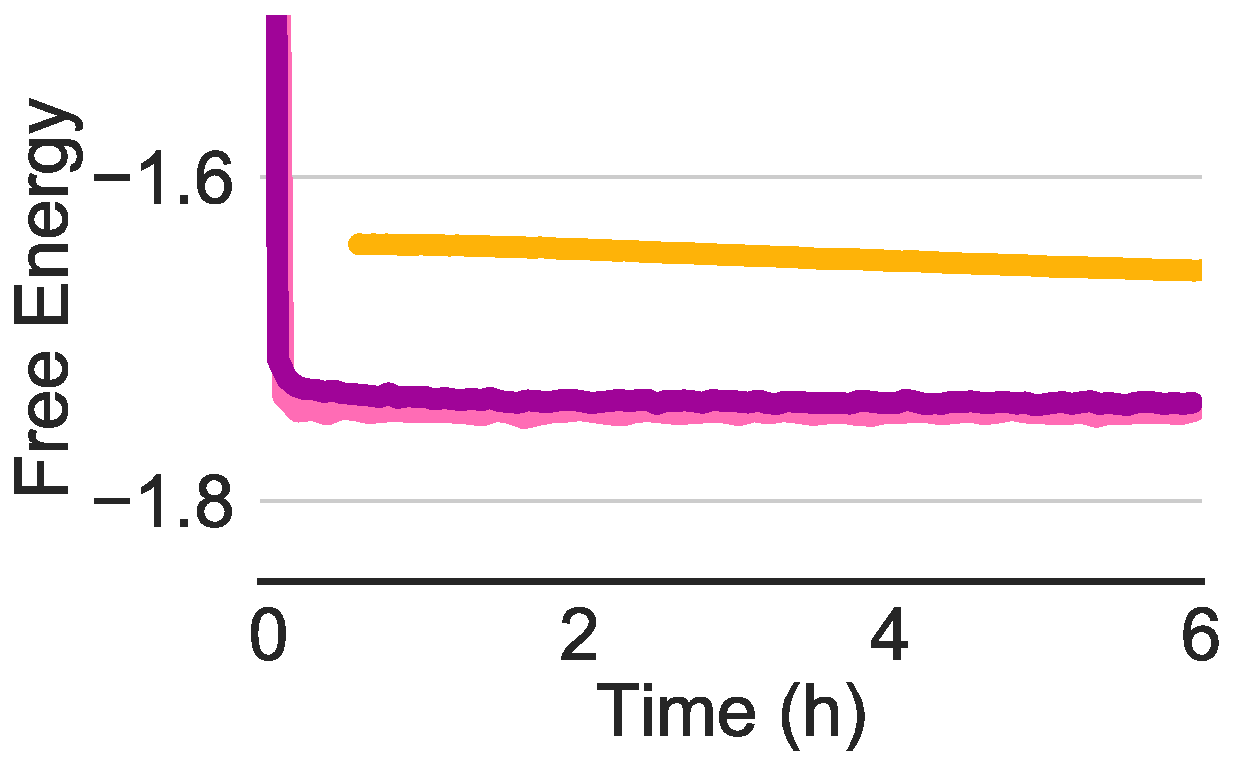
\includegraphics[width=\textwidth]{ch-hvm/fig/sk-large.pdf}
    % \caption{$\beta=0.4$}%
  \end{subfigure}
  % \hfill\hspace{\mywidth}%
  \begin{subfigure}[c]{0.3\linewidth}
    \centering
    % \raisebox{12mm}{
      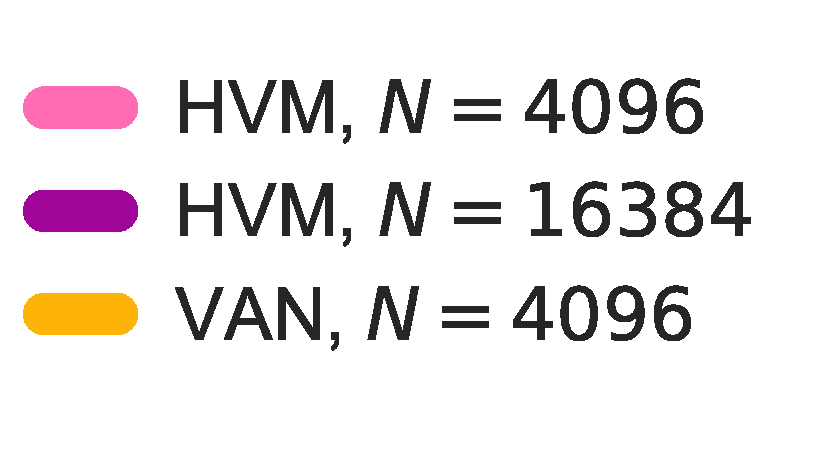
\includegraphics[width=\textwidth]{ch-hvm/fig/legend-sk}
    % }
  \end{subfigure}
  \hspace*{\fill}%
  % \vspace{-0.5cm}
  \caption[\textsc{hvm}s applied to the Sherrington-Kirkpatrick model]{\textbf{\Acrfullpl{hvm} scale to larger systems than \acrfull{van} models \citep{wu2019solving} when fit to the Sherrington-Kirkpatrick model using \acrlong{vi}.} (Lower is better, as the variational lower bound yields an upper bound on the free energy.) For the system with $N=4096$ variables the \gls{van} method completed fewer than ten iterations, and with $N=16384$ did not complete a single iteration.}
  \label{fig:sk}
\end{figure*}